%%%%%%%%%%%%%%%%%%%%%%%%%%%%%%%%%%%%%%%%%%%%%%%%%%%%%%%%%%%%%%%%%%%%%%%%%%%%%%%%
% ISE Lab -- Topic
% Giovanni Ciatto
% Alma Mater Studiorum - Università di Bologna
% mailto:giovanni.ciatto@unibo.it
%%%%%%%%%%%%%%%%%%%%%%%%%%%%%%%%%%%%%%%%%%%%%%%%%%%%%%%%%%%%%%%%%%%%%%%%%%%%%%%%
%\documentclass[handout]{beamer}\mode<handout>{\usetheme{default}}
%
\documentclass[presentation]{beamer}\mode<presentation>{\usetheme{AMSBolognaFC}}
%\documentclass[handout]{beamer}\mode<handout>{\usetheme{AMSBolognaFC}}
%%%%%%%%%%%%%%%%%%%%%%%%%%%%%%%%%%%%%%%%%%%%%%%%%%%%%%%%%%%%%%%%%%%%%%%%%%%%%%%%
\usepackage{phd-defense}
% version
\newcommand{\versionmajor}{0}
\newcommand{\versionminor}{3}
\newcommand{\versionpatch}{0}
\version{\versionmajor.\versionminor.\versionpatch}
%%%%%%%%%%%%%%%%%%%%%%%%%%%%%%%%%%%%%%%%%%%%%%%%%%%%%%%%%%%%%%%%%%%%%%%%%%%%%%%%

\school{\unibo}
%
\schoolShort{\uniboShort}
%
\programme{PhD Programme in `Data Science and Computation'}
%
\programmeShort{DS\&C}
%
\title[Role of CL in DS]{On the role of Computational Logic in Data Science}
%
\subtitle{Representing, Learning, Reasoning, and Explaining Knowledge}
%
\candidate{Giovanni Ciatto}
\candidateShort{G. Ciatto}
\candidateEmail{giovanni.ciatto@unibo.it}
%
\supervisor{Prof. Andrea Omicini}
\supervisorShort{A. Omicini}
\supervisorEmail{andrea.omicini@unibo.it}
%
\coordinator{Prof. Andrea Cavalli}
\coordinatorShort{A. Cavalli}
\coordinatorEmail{andrea.cavalli@unibo.it}
%
\contestsector{09/H1 -- Sistemi di Elaborazione delle Informazioni}
%
\scientificsector{ING-INF/05 -- Sistemi di Elaborazione delle Informazioni}
%
\cycle{XXXIII}
%
\examdate{June 16, 2022}
%
\examdateShort{2022-06-16}

\makeinfo

%%%%%%%%%%%%%%%%%%%%%%%%%%%%%%%%%%%%%%%%%%%%%%%%%%%%%%%%%%%%%%%%%%%%%%%%%%%%%%%%
\begin{document}
%%%%%%%%%%%%%%%%%%%%%%%%%%%%%%%%%%%%%%%%%%%%%%%%%%%%%%%%%%%%%%%%%%%%%%%%%%%%%%%%

%/////////
\frame{\titlepage}
%/////////

%%===============================================================================
\section*{Outline}
%%===============================================================================
%
%%/////////
\frame[c]{\tableofcontents[hideallsubsections]}
%%/////////

%===============================================================================
\section{Candidate Presentation}
%===============================================================================

\begin{frame}{About Me}
    \begin{itemize}
        \item Bachelor in \alert{Software Engineering} (2011--2014)

        \vfill
        
        \item Master in \alert{Computer Science and Engineering} (2014--2017)

        \vfill
        
        \item PhD in \alert{Data Science and Computation} (2017--2022)
        %
        \begin{itemize}
            \item with a focus on foundational \alert{Artificial Intelligence}
        \end{itemize}

        \vfill
        
        \item Currently:
        %
        \begin{itemize}
            \item research fellow at \disiShort{} (\uniboShort{})
            \item funded by the \alert{EXPECTATION} project\footnote{\url{http://www.chistera.eu/projects/expectation}}
            %
            \begin{itemize}
                \item where I am WP-leader
            \end{itemize}
        \end{itemize}
    \end{itemize}
\end{frame}

%===============================================================================
\section{Context, Motivation, and Goals}
%===============================================================================

\begin{frame}{Context}
    \begin{itemize}
        \item Era of \alert{data-driven} artificial intelligence (AI)
        %
        \begin{itemize}
            \item major availability of \alert{data} and \alert{computational resources}
            \item pervasive exploitation in science and in the industry
        \end{itemize}

        \vfill

        \item Deep entanglement among AI and \alert{data science} (DS)
        %
        \begin{itemize}
            \item both leveraging \alert{machine learning} to mine information from data
        \end{itemize}
        
        \vfill

        \item AI involves not only data-driven approaches
        %
        \begin{itemize}
            \item[eg] good old-fashioned AI (GOFAI), \alert{computational logic}\ccite{lloyd1990computational} (CL) 
        \end{itemize}

        \vfill
        
        \item Following a ``classical'' perspective, we distinguish among\ccite{explanation-aixia2020dp}
        %
        \begin{itemize}
            \item \alert{symbolic} AI $\approx$ CL $\rightarrow$ emulating humans' \alert{rational reasoning}
            \item \alert{\emph{sub}-symbolic} $\approx$ ML / DS  $\rightarrow$ emulating humans' \alert{intuition}
        \end{itemize}
    \end{itemize}
\end{frame}

\begin{frame}{Motivation}
    \begin{itemize}
        \item \alert{Limitation} of sub-symbolic AI are now becoming relevant \alert{issues}, e.g.
        %
        \begin{itemize}
            \item interpretability/\alert{explainability}\ccite{darpa2016-xai}
            \item data-greediness\ccite{CropperDM20}
            \item human-in-the-loop\ccite{Yao2018}
        \end{itemize}
        
        \vfill

        \item Symbolic and sub-symbolic have several \alert{complementarities}
        %
        \begin{itemize}
            \item[$\rightarrow$] integrating the two may lead to a better AI\ccite{Hoehndorf2017}
        \end{itemize}

        \vfill

        \item Long-standing interest in \alert{integrating} the two\ccite{IlkouK20}

        \vfill

        \item Interest in spotting (and overcoming) \alert{obstacles} preventing integration
        %
        \begin{itemize}
            \item either at the theoretical or technological level
        \end{itemize}
    \end{itemize}
\end{frame}

\begin{frame}{Goals}

    \emph{Foundational} goals:
    %
    \vfill
    %
    \begin{enumerate}
        \item \alert{comparing} DS and CL w.r.t. how they manage \alert{knowledge}
        %
        \begin{itemize}
            \item \alert{representation}
            \item acquisition (a.k.a. \alert{learning})
            \item inference (a.k.a. \alert{reasoning})
            \item transferring (a.k.a. \alert{explanation})
        \end{itemize}
        
        \vfill

        \item \alert{elicit} synergies and complementarities, and frictions w.r.t. \alert{integration}

        \vfill

        \item assess the \alert{technological gap} among the two
        %
        \begin{itemize}
            \item design \& \alert{prototype software} technologies for filling it
        \end{itemize}
    \end{enumerate}
\end{frame}

\begin{frame}{Organization of the Thesis}

    Two major parts, concerning the integration of CL and DS:
    %
    \vfill
    %
    \begin{block}{\textbf{Computational} perspective: \textbf{what} aspects can be integreted}
        \begin{enumerate}
            \item understand the \alert{analogies} and \alert{differences} among CL and DS
            \item derive a \alert{conceptual framework} bridging them
        \end{enumerate}
    \end{block}
    %
    \vfill
    %
    \begin{block}{\textbf{Technological} perspective: \textbf{how} to integrate them}
        \begin{enumerate}\setcounter{enumi}{2}
            \item evaluate the current \alert{state of the art} of AI \alert{technologies}
            \item propose the notion of \alert{logic ecosystem} to support integration
            \item discuss the \alert{reification} of logic ecosystems into \alert{software}
        \end{enumerate}
    \end{block}

\end{frame}

%===============================================================================
\section{Background}
%===============================================================================

% \subsection{Data Science}

\begin{frame}{Data Science\ccite{Hoehndorf2017}}
    \begin{itemize}
        \item Novel discipline laying at the intersection among \ldots
        %
        \begin{itemize}
            \item[] \ldots Computer Science, Statistics, AI, Software Engineering
        \end{itemize}
        
        \vfill 
        
        \item Focus on modelling the world following a \alert{data-driven} approach
        %
        \begin{itemize}
            \item possibly, by leveraging \alert{Machine Learning} (ML) or Data Mining
        \end{itemize}
        
        \vfill

        \item Pros/cons:
        %
        \begin{itemize}
            \item[$+$] data-driven $\rightarrow$ bottom-up $\rightarrow$ adherence to reality
            \item[$+$] scalable algorithms for learning
            \item[$\sim$] flexibility w.r.t. errors in the data or in the model
            \item[$-$] reliance on poorly interpretable models
            \item[$-$] simple, stimulus--response form of inference
        \end{itemize}
    \end{itemize}
\end{frame}

% \subsection{Computational Logic}

\begin{frame}{Computational Logic\ccite{lloyd1990computational}}
    \begin{itemize}
        \item Well-established discipline laying at the intersection among CS, logic, and mathematics
        
        \vfill 
        
        \item Focus on using formal logics as a means for computing
        %
        \begin{itemize}
            \item hence, on making software systems able to reason, rationally
        \end{itemize}
        
        \vfill

        \item Pros/cons:
        %
        \begin{itemize}
            \item[$+$] powerful, ``rational'' form of inference
            \item[$+$] reliance on machine- and human-interpretable representations
            \item[$\sim$] crisp and exact representations and decisions
            \item[$-$] reliance on poorly scalable, often untractable, or undecidable algorithms
            \item[$-$] top-down approach to knowledge, possibly detached from reality
        \end{itemize}
    \end{itemize}
\end{frame}

%===============================================================================
\section{Computational Perspective (What)}
%===============================================================================

\begin{frame}{Overview}
    Four major aspects to be analysed:
    %
    \vfill
    %
    \begin{description}
        \item[Representation:] how are data and knowledge expressed
        %
        \begin{itemize}
            \item[\ldots] and made available to computers / humans
        \end{itemize}
        
        \vfill

        \item[Learning:] how is novel re-usable knowledge distillied from data
        
        \vfill

        \item[Inference:] how are predictions drawn from prior knowledge
        
        \vfill

        \item[Explanation:] how is information transferred to another (possibly human) agent

    \end{description}
\end{frame}

\subsection{Representation}

\begin{frame}[allowframebreaks]{CL vs. DS -- Representation}
    \begin{block}{DS leverages on sub-symbolic representations}
        \begin{itemize}
            \item $\begin{cases}
                \alert{\text{data}} \rightarrow \text{numeric datasets of \alert{fixed} size}
                \\
                \alert{\text{knowledge}} \rightarrow \text{\alert{opaque} models mimicking \alert{real functions}}
            \end{cases}$
            \item issues may arise from \alert{recursive}, or \alert{depth-unlimited} concepts
            \item representations may easily become \alert{unintelligible} 
        \end{itemize}
    \end{block}

    \begin{block}{CL leverages on the language of logic}
        \begin{itemize}
            \item several \alert{logic formalisms} available
            \begin{itemize}
                \item \alert{expressivity--tractability} trade-off\ccite{LevesqueB87}
                \item good trade-off\ccite{Makowsky1987} provided by \alert{Horn clauses}\ccite{Horn1951}
            \end{itemize}
            \item coherent representation of both data and knowledge via relations
            \item both human- and machine-interpretable
            \item support for intensional representations
            \item support for recursive / structured information
            \end{itemize}
    \end{block}
\end{frame}

\begin{frame}{What does `symbolic' actually mean?}
    \begin{block}{\textbf{Symbolic} representations of knowledge should\cccite{Gelder90}}
        \begin{itemize}
            \item involve a \alert{set of symbols},
            \item which can be combined in (possibly) \alert{infinitely many} ways, 
            \item following precise \alert{syntactical} rules, and
            \item where both elementary and combined symbols have \alert{meaning}
            %
            \begin{itemize}
                \item[ie] \alert{each} symbol can be mapped into some entity from the domain at hand.
            \end{itemize}
        \end{itemize}
    \end{block}

    \begin{alertblock}{Opposite notion: \textit{distributed} representations (a.k.a. \textbf{sub-symbolic})}
        \begin{itemize}
            \item where symbols \alert{alone} have no meaning\ldots
            \item \ldots unless it is considered along with its \alert{neighbourhood}
            %
            \begin{itemize}
                \item[ie] any other symbol which is \alert{close} (according to some notion of closeness)
            \end{itemize}
        \end{itemize}
    \end{alertblock}
\end{frame}

\subsection{Learning}

\begin{frame}[allowframebreaks]{CL vs. DS -- Learning}
    \begin{block}{Similar formulation}
        \begin{itemize}
            \item search the best hypothesis in an hypothesis space
            \item human-in-the-loop required to chose the hypothesis space
            \item automatic procedures for exploring the hypothesis space
            \item learning as non-deterministic (possibly stochastic) process
        \end{itemize}
    \end{block}

    \begin{block}{Different implementations}
        \begin{itemize}
            \item DS $\rightarrow$ numeric data $\rightarrow$ differentiable hypothesis space
            %
            \begin{itemize}
                \item search by gradient descent
                \item fuzzy constraints, fuzzy outcomes
                \item support for hardware acceleration via TPU
            \end{itemize}

            \item CL $\rightarrow$ symbolic knowledge bases $\rightarrow$ discrete search space
            %
            \begin{itemize}
                \item search by inductive logic programming\ccite{CropperD2020}
                \item crisp constraints, consistent outcomes
                \item virtual support for concurrency (unexplored)
            \end{itemize}
        \end{itemize}
    \end{block}

    \begin{block}{Different expectations}
        \begin{itemize}
            \item DS learns numeric functions
            \item CL learns symbolic relations
            %
            \begin{itemize}
                \item[aka] logic programs 
                %
                \begin{itemize}
                    \item possibly recursive, intelligible, and expressive
                \end{itemize}
            \end{itemize}
        \end{itemize}
    \end{block}
\end{frame}

\subsection{Inference}

\begin{frame}%[allowframebreaks]
    \frametitle{CL vs. DS -- Inference}

    \begin{block}{DS feeds trained models with unseen data}
        \begin{itemize}
            \item \alert{inference} $\approx$ quick \& dirty responses to stimuli
            \item models as black-box functions
        \end{itemize}
    \end{block}

    \begin{block}{CL applies inference rules in a principled way}
        \begin{itemize}
            \item \alert{inference} $\approx$ reasoning $\approx$ drawing conclusions from prior knowledge 
            \item several ways of reasoning:
            %
            \begin{itemize}
                \item deductive, e.g. SLD\ccite{Kowalski1976} and Prolog\ccite{Korner2020HistoryFuturePrologTPLP}
                \item inductive, e.g. ILP\ccite{CropperDM20}
                \item abductive, e.g. IFF\ccite{FungK97}
                \item probabilistic, e.g. LPAD\ccite{VennekensVB04} 
            \end{itemize}
            \item reasoners as expert oracles 
            %
            % \begin{itemize}
            %     \item users may either observe the result or the reasoning process
            % \end{itemize}
            \item reasoning requires computational time/space
        \end{itemize}
    \end{block}
\end{frame}

\subsection{Explanation}

\begin{frame}%[allowframebreaks]
    \frametitle{CL vs. DS -- Explaining}

    \begin{block}{The \textbf{opacity} problem in ML}
        \begin{itemize}
            \item due to sub-symbolic models being black boxes\ccite{Lipton18}
            \item need to \alert{explain} how they work $\rightarrow$ XAI\ccite{darpa2016-xai}
            \item models as black-box functions
        \end{itemize}
    \end{block}

    \begin{alertblock}{Symbolic systems are inherently interpretable}
        \begin{itemize}
            \item as symbols are meant to carry meaning for users
            \item insight: convert sub-symbolic models into symbolic ones
        \end{itemize}
    \end{alertblock}
\end{frame}

\begin{frame}[allowframebreaks]{An abstract framework for XAI\ccite{agentbasedxai-extraamas2020}}

    \begin{center}
        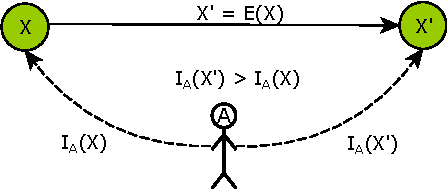
\includegraphics[width=.5\linewidth]{figures/framework.pdf}
    \end{center}
    %
    \begin{itemize}
        \item[$X$] object to be explained
        \item[$A$] observer agent
        \item[$I_A(\cdot)$] a function ``measuring'' the ``degree of interpretability'' of $X$, w.r.t. $A$
        \item[$E(\cdot)$] an \alert{explanation} function, mapping objects into (different) objects      
        \item[$X'$] the \alert{result} of the explanation, i.e. a \alert{more-interpretable} object
    \end{itemize}
    
    \begin{block}{Key points}
        \begin{itemize}
            \item interpretation is \alert{subjective}
            \item `interpretability' does not need to be measurable
            \item explanation $\approx$ search of a \alert{surrogate} interpretable model
        \end{itemize}
    \end{block}
\end{frame}

\begin{frame}[allowframebreaks]{Symbolic Knowledge Extraction (SKE)}
    \begin{columns}
        \begin{column}{0.19\linewidth}
            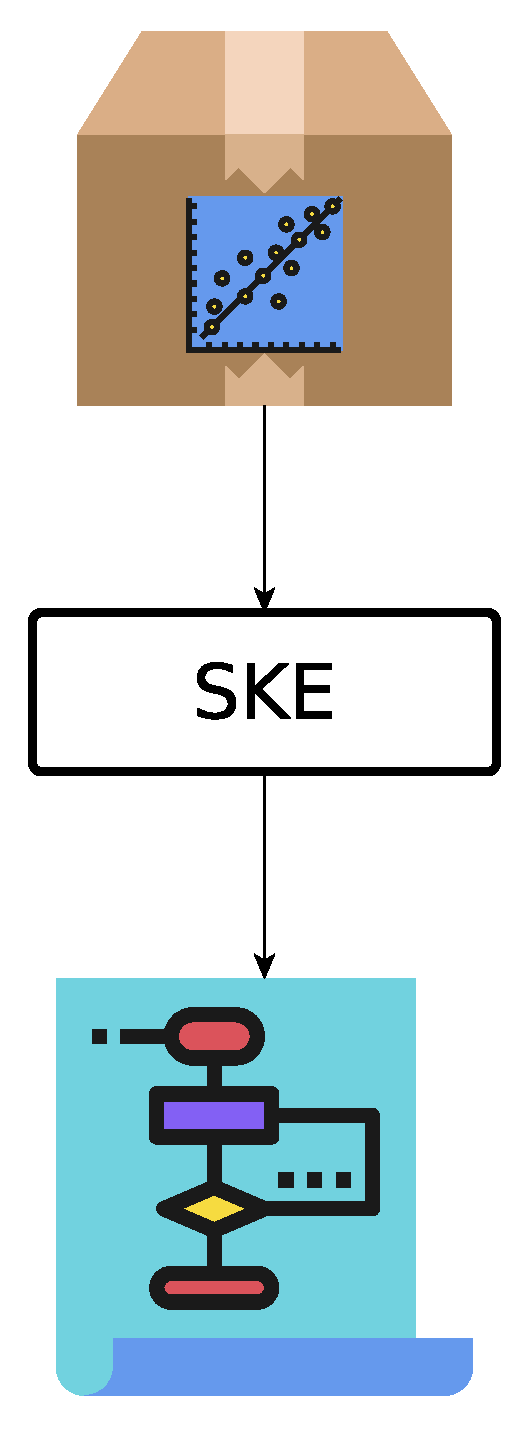
\includegraphics[width=\linewidth]{figures/ske.pdf}
        \end{column}
        \hfill
        \begin{column}{0.8\linewidth}
            \begin{block}{Insight}
                \begin{itemize}
                    \item search of a \alert{surrogate} interpretable model\ldots
                    \medskip
                    \item \ldots consisting of \alert{symbolic knowledge}
                \end{itemize}
            \end{block}
        \end{column}
    \end{columns}

    \framebreak

    Example:
    %
    \begin{columns}
        \begin{column}{.43\linewidth}
            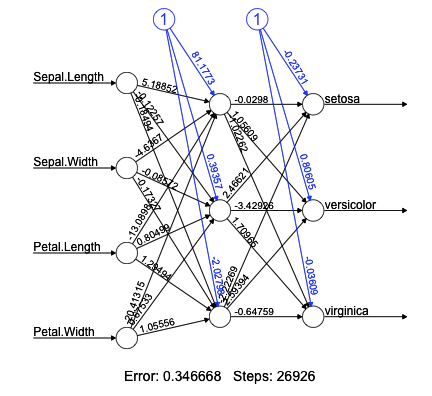
\includegraphics[width=\linewidth]{figures/nn-iris.png}
        \end{column}
        $\rightarrow$
        \begin{column}{.53\linewidth}\small
            \[ 
                \begin{array}{l}
                    \variable{Class} = \functor{setosa} \leftarrow \variable{PetalWidth} \leq 1.0 \fullstop
                    \\
                    \\
                    \variable{Class} = \functor{versicolor} \leftarrow \variable{PetalLength} > 4.9 \\ 
                        \qquad  \wedge\ \variable{SepalWidth} \in [2.9,\ 3.2] \fullstop
                    \\
                    \variable{Class} = \functor{versicolor} \leftarrow  \variable{PetalWidth} > 1.6 \fullstop
                    \\
                    \\
                    \variable{Class} = \functor{virginica} \leftarrow \variable{SepalWidth} \leq 2.9 \fullstop
                    \\
                    \\
                    \variable{Class} = \functor{virginica} \leftarrow \\ 
                        \qquad \variable{SepalLength} \in [5.4,\ 6.3] \fullstop
                    \\
                    \variable{Class} = \functor{virginica} \leftarrow \\ 
                        \qquad \variable{PetalWidth} \in [1.0,\ 1.6] \fullstop
                \end{array}    
            \]
        \end{column}
    \end{columns}
\end{frame}



%===============================================================================
\section{Technological Perspective (How)}
%===============================================================================

\begin{frame}{Overview}
    \begin{enumerate}
        \item Survey the state of the art of AI technologies
        
        \vfill

        \item Design and implement the notion of logic ecosystem 
        
        \vfill

        \item Extend the ecosystem to support hybrid inference, learning, and explanation
    \end{enumerate}
\end{frame}

\subsection{Technology State of the Art}

\begin{frame}{Current state of technology}
    \begin{itemize}

        \item Authored many surveys concerning logic-based technologies (LBT)
        %
        \begin{itemize}
            \item[eg] \ccite{xaisurvey-ia14,lptech4mas-jaamas35,coordination-jlamp2020,logictech-information11}
        \end{itemize}
        
        \vfill

        \item Few mature technologies, many proof of concepts
        
        \vfill

        \item Plenty of technology silos
        %
        \begin{itemize}
            \item well-engineered, optimised, and purpose-specific technologies\ldots
            \item \dots yet poorly interoperable and portable
        \end{itemize}
        
        \vfill

        \item Prolog\ccite{Korner2020HistoryFuturePrologTPLP} as the most prominent LBT
        
        \vfill

        \item Conversely, DS-oriented technologies are flourishing
        %
        \begin{itemize}
            \item an ecosystem of interoperable and portable technologies is emerging
            %
            \begin{itemize}
                \item[eg] \scikit{}, Tensorflow, Pandas, Matplotlib, etc.
            \end{itemize}
        \end{itemize}
    \end{itemize}
\end{frame}

\begin{frame}{Need for a Logic Ecosystem}
    \begin{itemize}
        \item Set of loosely coupled software tools
        %
        \begin{itemize}
            \item supporting individual aspects of CL
            \item and their hybridisation with DS
        \end{itemize}

        \vfill

        \item usable as either a library or a CLI/GUI tool
        
        \vfill

        \item interoperable with as many software tools as possible
        
        \vfill

        \item portable on as many software platforms/runtimes as possible
        
        \vfill

        \item to be incrementally extended by the CL or DS communities
        %
        \begin{itemize}
            \item recalling the intricacies of research-oriented software development
        \end{itemize}
    \end{itemize}
\end{frame}

\subsection{The \twopkt{} Logic Ecosystem}

\begin{frame}{Overview}
    \begin{block}{The \twopkt{} project \hfill (\url{https://github.com/tuProlog/2p-kt})}
        \begin{itemize}
            \item Kotlin-based implementation of a logic ecosystem
            \item multi-platform, multi-OS, multi-paradigm
        \end{itemize}
    \end{block} 

    \begin{center}
        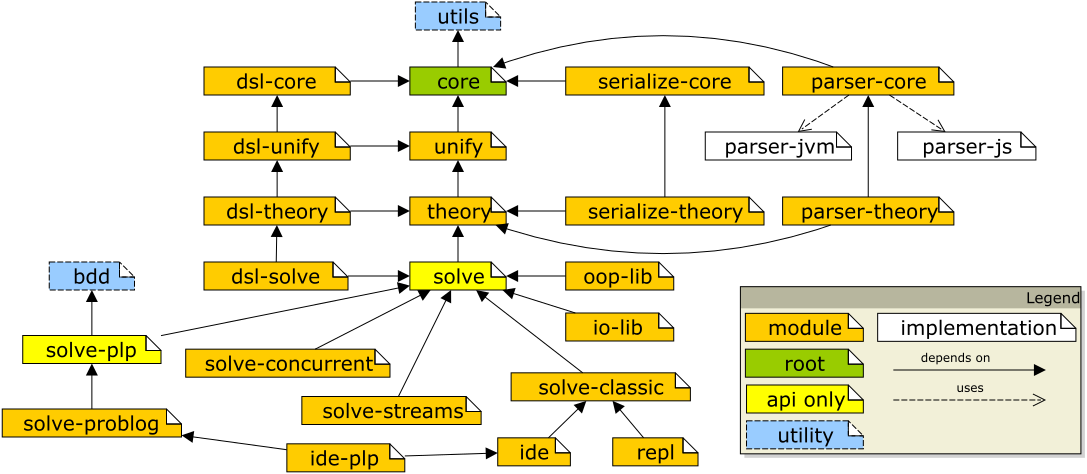
\includegraphics[width=.7\linewidth]{figures/project-map.png}    
    \end{center}

    \begin{multicols}{2}
        \begin{itemize}\small
            \item knowledge representation
            
            \item \ldots and storage
            
            \item \ldots and parsing/presentation

            \item Prolog-like inference support
            %
            \item \ldots or concurrent / probabilistic
            
            \item CLI / GUI / testing facilities
        \end{itemize}
    \end{multicols}
\end{frame}

%===============================================================================
\section{Conclusions and Future Works}
%===============================================================================

\begin{frame}{First Exercise}
    \begin{block}{Goal}
        Goal here
    \end{block}
    %
    \begin{itemize}
        \item further info here
    \end{itemize}
\end{frame}

%===============================================================================
\section*{}
%===============================================================================

%/////////
\frame{\titlepage}
%/////////

%===============================================================================
\section*{\refname}
%===============================================================================

%%%%
\setbeamertemplate{page number in head/foot}{}
%/////////
% \begin{frame}[c,noframenumbering]{\refname}
\begin{frame}[t,allowframebreaks,noframenumbering]{\refname}
%	\tiny
    \scriptsize
%	\footnotesize
    \bibliographystyle{apalike-AMS}
    \bibliography{phd-defense,my-papers}
\end{frame}
%/////////

%%%%%%%%%%%%%%%%%%%%%%%%%%%%%%%%%%%%%%%%%%%%%%%%%%%%%%%%%%%%%%%%%%%%%%%%%%%%%%%%
\end{document}
%%%%%%%%%%%%%%%%%%%%%%%%%%%%%%%%%%%%%%%%%%%%%%%%%%%%%%%%%%%%%%%%%%%%%%%%%%%%%%%%
